\chapter*{Введение}
\addcontentsline{toc}{chapter}{Введение}



\chapter{Основная часть}

\section{Характеристика организации}

ПАО «МАК «Вымпел» — предприятие российской оборонной про-
мышленности в области ракетно-космической обороны. Входит в состав АО «Концерн «ВКО «Алмаз-Антей». Корпорация «Вымпел» отвечает за широкий комплекс наукоемких работ, связанных с проектированием, созданием, испытаниями и развитием систем, решающих задачи предупреждения о ракетном нападении (СПРН), противоракетной обороны (ПРО) и контроля космического пространства (СККП), создает и совершенствует программно-алгоритмическое обеспечение для одновременной обработки гиперобъемной информации и визуализации ее результатов на командных пунктах этих систем. 

Все системы и средства РКО работают в полностью автоматическом режиме, в реальном масштабе времени, с возможностью одновременного управления с командных пунктов. Существенную долю объема работ корпорации составляет наукоемкая продукция, разрабатываемая в интересах российских и иностранных заказчиков.\cite{about}

\section{Задание на практику}

В последнее время происходит быстрый рост количества космических аппаратов, в основном за счет разворачивания группировок на низких орбитах.\cite{Фатеев2014} Это предполагает оптимизацию планирования наблюдений наземными средствами.

В рамках практики было предложено реализовать ряд алгоритмов планирования наблюдений за спутниками. Данные в виде времени видимости спутников за 150 дней были предоставлены организацией.

\section{Алгоритмы планирования}

Были рассмотрены и реализованы следующие алгоритмы планирования:

\begin{enumerate}
	\item LIHP (last in hight priority) В случае коллизии наблюдается спутник, который последним попал в зону видимости станции мониторинга. Для этого алгоритма станция РТМ в случае коллизии переходит к наблюдению нового спутника.
	\item FIHP (first in high priority). В случае коллизии наблюдается спутник, который первым попал в зону видимости станции мониторинга. Для этого алгоритма, станция в случае коллизии продолжает следить за спутником, не переходя к наблюдению нового. После этого выбирается спутник, который первым вошел в область наблюдения при коллизии.
	\item RW (random walk, случайные блуждания). В данном алгоритме при возникновении коллизии выбор спутника, за которым будет вестись наблюдение, осуществляется по марковскому правилу принятия решений. В случае возникновения коллизии среди спутников одного приоритета, спутник выбирается случайно с вероятностью $P_i(t) = \frac{1}{N}$, где $N$ – количество спутников участвующих в коллизии.
	\item Алгоритм принятия решения с учетом всего интервала планирования. Алгоритм состоит из 6 основных шагов:
	\begin{enumerate}
		\item Добавление в план наблюдения интервалов времени в которых отсутствует коллизия.\label{step1}
		\item Расчёт среднего времени наблюдения спутника $t_{mean}$ \label{step2}
		\item Спутники сортируются по возрастанию потенциальной длительности наблюдения $t_i^{pot}$ \label{step3}
		\item Производится сравнение потенциального времени наблюдения каждого космического аппарата со средним временем наблюдения $t_mean$. Если $t_i^{pot}$, то есть потенциальное время наблюдения спутника меньше или равно среднему, то все интервалы видимости соответствующего спутника добавляются в план наблюдения и алгоритм переходит к шагу \ref{step6}. Если потенциальное время наблюдения спутника больше среднего времени наблюдения спутника, то алгоритм переходит к шагу \ref{step5}. \label{step4}
		\item Перерасчет среднего (при необходимости). На этом шаге пересчитывается среднее время наблюдения и добавляется в расписание время наблюдения спутника с самым маленьким интервалом видимости из спутников, которые еще не были добавлены в расписание. Если таких спутников несколько, то выбирается тот, у которого меньший интервал времени уже добавлен в расписание. Если в этом случае спутников несколько, выбирается произвольный.\label{step5}
		\item Переход к следующему спутнику, \ref{step3} алгоритма.\label{step6}
	\end{enumerate}
	\item Алгоритм принятия решения с учетом всего интервала планирования, а также приоритетности космических аппаратов. Данный алгоритм схож с алгоритмом, описанным в пункте выше, однако учитывает приоритет космических аппаратов. В реализации были заданы 3 приоритета - 3, 2, 1, где 3 - самый высокий, а 1 - самый низкий.
\end{enumerate}

\subsection{Результаты планирования}

Ниже приведены гистограммы результатов планирования наблюдений реализованными алгоритмами.

\begin{figure}[H]
	\centering
	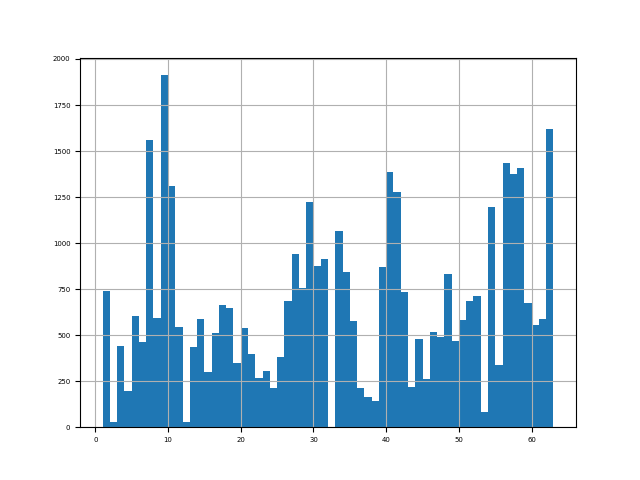
\includegraphics[width=0.8\textwidth]{assets/LIHP.png}
	\caption{Общее время наблюдения каждого спутника при использовании алгоритма планирования LIHP}
\end{figure}

\begin{figure}[H]
	\centering
	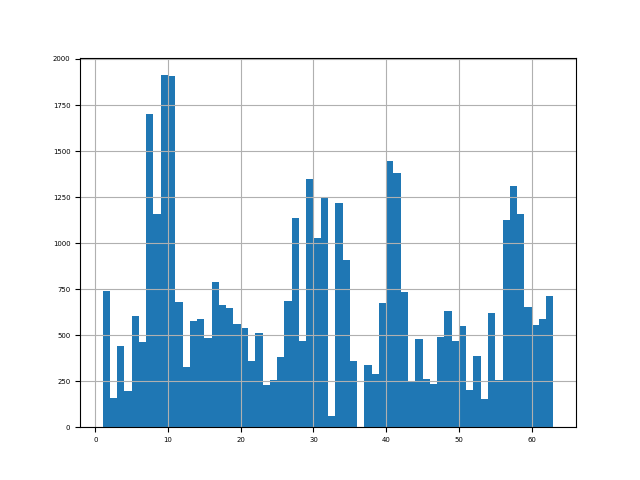
\includegraphics[width=0.8\textwidth]{assets/FIHP.png}
	\caption{Общее время наблюдения каждого спутника при использовании алгоритма планирования FIHP}
\end{figure}

\begin{figure}[H]
	\centering
	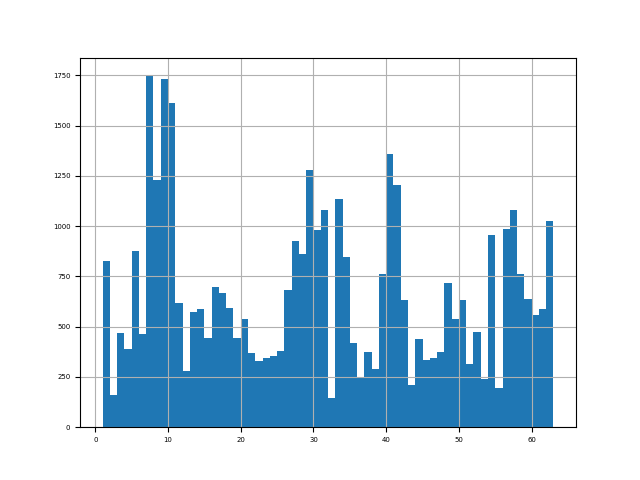
\includegraphics[width=0.8\textwidth]{assets/RW.png}
	\caption{Общее время наблюдения каждого спутника при использовании алгоритма планирования RW}
\end{figure}

\begin{figure}[H]
	\centering
	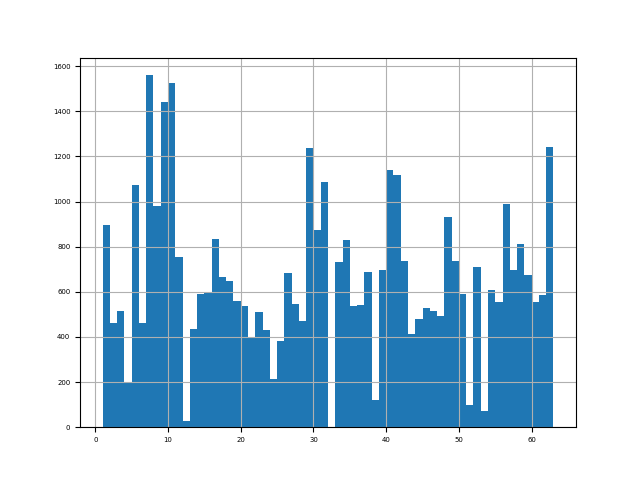
\includegraphics[width=0.8\textwidth]{assets/interv.png}
	\caption{Общее время наблюдения каждого спутника при использовании алгоритма планирования с учетом всего интервала наблюдения}
\end{figure}

\begin{figure}[H]
	\centering
	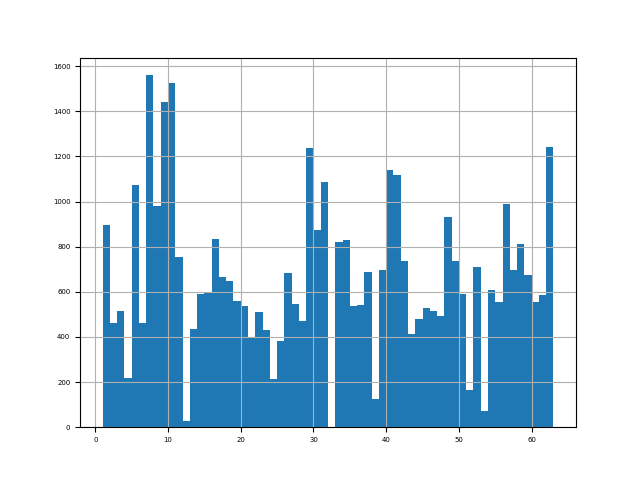
\includegraphics[width=0.8\textwidth]{assets/modif.png}
	\caption{Общее время наблюдения каждого спутника при использовании алгоритма планирования с учетом приоритета космических аппаратов}
\end{figure}

\section{Сравнительный анализ алгоритмов планирования}

В таблице \ref{tab:time} представлено среднее время выполнения каждого реализованного алгоритма, в которой 

\begin{itemize}
	\item LIHP - last in hight priority;
	\item FIHP - first in high priority;
	\item RW - random walk;
	\item interv - алгоритм принятия решения с учетом всего интервала планирования;
	\item modif - модифицированный алгоритм принятия решения с учетом всего интервала планирования и приоритетности космических аппаратов.
\end{itemize}

\captionsetup{singlelinecheck = false, justification=raggedleft}
\begin{table}[H]
	\centering
	\caption{Среднее время выполнения, с}
	\renewcommand{\arraystretch}{1.5}
	\resizebox{\textwidth}{!}{
	\begin{tabularx}{1\textwidth} { 
			| >{\centering\arraybackslash}X 
			| >{\centering\arraybackslash}X 
			| >{\centering\arraybackslash}X 
			| >{\centering\arraybackslash}X 
			| >{\centering\arraybackslash}X | }
		\hline
		LIHP & FIHP & RW & interv & modif \\
		\hline
		14.9167 & 7.8685 & 22.8472 & 30.0623 & 58.8573 \\
		\hline
	\end{tabularx}
	}
\label{tab:time}
\end{table}

\subsection{Выводы}

На основе полученных данных можем сделать следующие выводы:

\begin{enumerate}
	\item Алгоритмы LIHP, FIHP, RW не гарантируют равномерность распределения по времени. При этом в алгоритмах FIHP и RW возникает вероятность пропуска спутника, который наблюдается кратковременно одновременно с другим спутником.
	\item Алгоритм, учитывающий все время планирования, работает почти в 4.3 раза быстрее алгоритма FIHP, однако он обеспечивает выравнивание времени наблюдения каждого КА и при этом достигается максимально возможное общее время наблюдения.
	\item Модифицированный алгоритм планирования, учитывающий не только все время планирования, но и приоритетность космических аппаратов, работает почти в 7.55 раз медленнее алгоритма FIHP и в 1.96 раз медленнее алгоритма планирования, учитывающего только общее время наблюдений.
\end{enumerate}

\chapter*{Заключение}
\addcontentsline{toc}{chapter}{Заключение}

\addchap{Список литературы}
~~~ % костыль чек
\printbibliography[heading=none]
